% !TeX spellcheck = ru_RU
% !TEX root = vkr.tex

\section{Эксперимент}

\subsection{Условия эксперимента}

Экспериментальное исследование проводилось на трёх аппаратных платформах: двух одноплатных компьютерах на базе архитектуры RISC-V (Banana Pi BPI-F3 и StarFive VisionFive 2) и одной референсной платформе на базе архитектуры x86-64 со встроенной графикой Intel (Intel Core i9-12900H с Intel Iris Xe Graphics).

Характеристики платформ:
\begin{itemize}
    \item \textbf{Banana Pi BPI-F3}: SpacemiT K1 (8 ядер RISC-V @ 2.0 ГГц), IMG BXE-2-32 GPU, 16 ГБ LPDDR4-2666;
    \item \textbf{StarFive VisionFive 2}: JH7110 (4 ядра RISC-V @ 1.5 ГГц), IMG BXE-4-32 MC1 GPU, 8 ГБ LPDDR4-2800;
    \item \textbf{Intel Iris Xe}: Intel Core i9-12900H (14 ядер @ до 5.0 ГГц), Intel Iris Xe Graphics (96 EU), 24 ГБ DDR5-4800.
\end{itemize}

Для каждой конфигурации параметров и каждого ядра выполнялось по 100 прогонов операции умножения матриц. Измерялось только время выполнения OpenCL ядра, без учёта времени на подготовку данных, их копирование в память устройства и обратно. Это позволило получить чистую оценку вычислительной производительности различных реализаций алгоритма. Для обработки результатов использовалось среднее арифметическое значение времени выполнения.

Для обеспечения стабильности измерений на RISC-V платформах использовалось пассивное охлаждение, частоты процессоров работали в штатном режиме с динамическим управлением. Скрипты для автоматизации тестирования и обработки результатов доступны в форке репозитория MyGEMM~\cite{mygemm_repo_test}.

\subsection{Тестовые данные}

В качестве тестовых данных использовались квадратные матрицы размером $1024 \times 1024$ элементов типа \texttt{float} (32-бит). Размер матриц был выбран достаточно большим для выявления различий в производительности различных оптимизаций, но при этом умещающимся в память всех тестируемых устройств.

Тестировались 11 ядер библиотеки MyGEMM (от наивной реализации до продвинутых оптимизаций) с различными наборами параметров конфигурации. Для ядер 1--3 варьировался параметр TS (Tile Size) со значениями из множества \{8, 16\}. Попытки запуска с TS=32 приводили к ошибке выполнения ``Invalid work group size''.

Для ядер 4--10 тестировались комбинации параметров TSM и TSN из множества \{32, 64, 128\} с соответствующими значениями WPTM и WPTN, что дало 9 уникальных конфигураций для каждого ядра. Ядро 11 имеет фиксированную конфигурацию параметров, определённую реализацией clBLAS.

Все конфигурации параметров были подобраны с учётом ограничения максимального размера рабочей группы в 32 потока на RISC-V платформах.

\subsection{Результаты тестирования MyGEMM}

Результаты экспериментов с библиотекой MyGEMM представлены на рисунках~\ref{fig:perf_bananapi}--\ref{fig:perf_intelxe} для каждой из тестируемых платформ. На графиках показано среднее время выполнения операции умножения матриц в секундах для различных ядер и конфигураций параметров.

\begin{figure}[H]
\centering
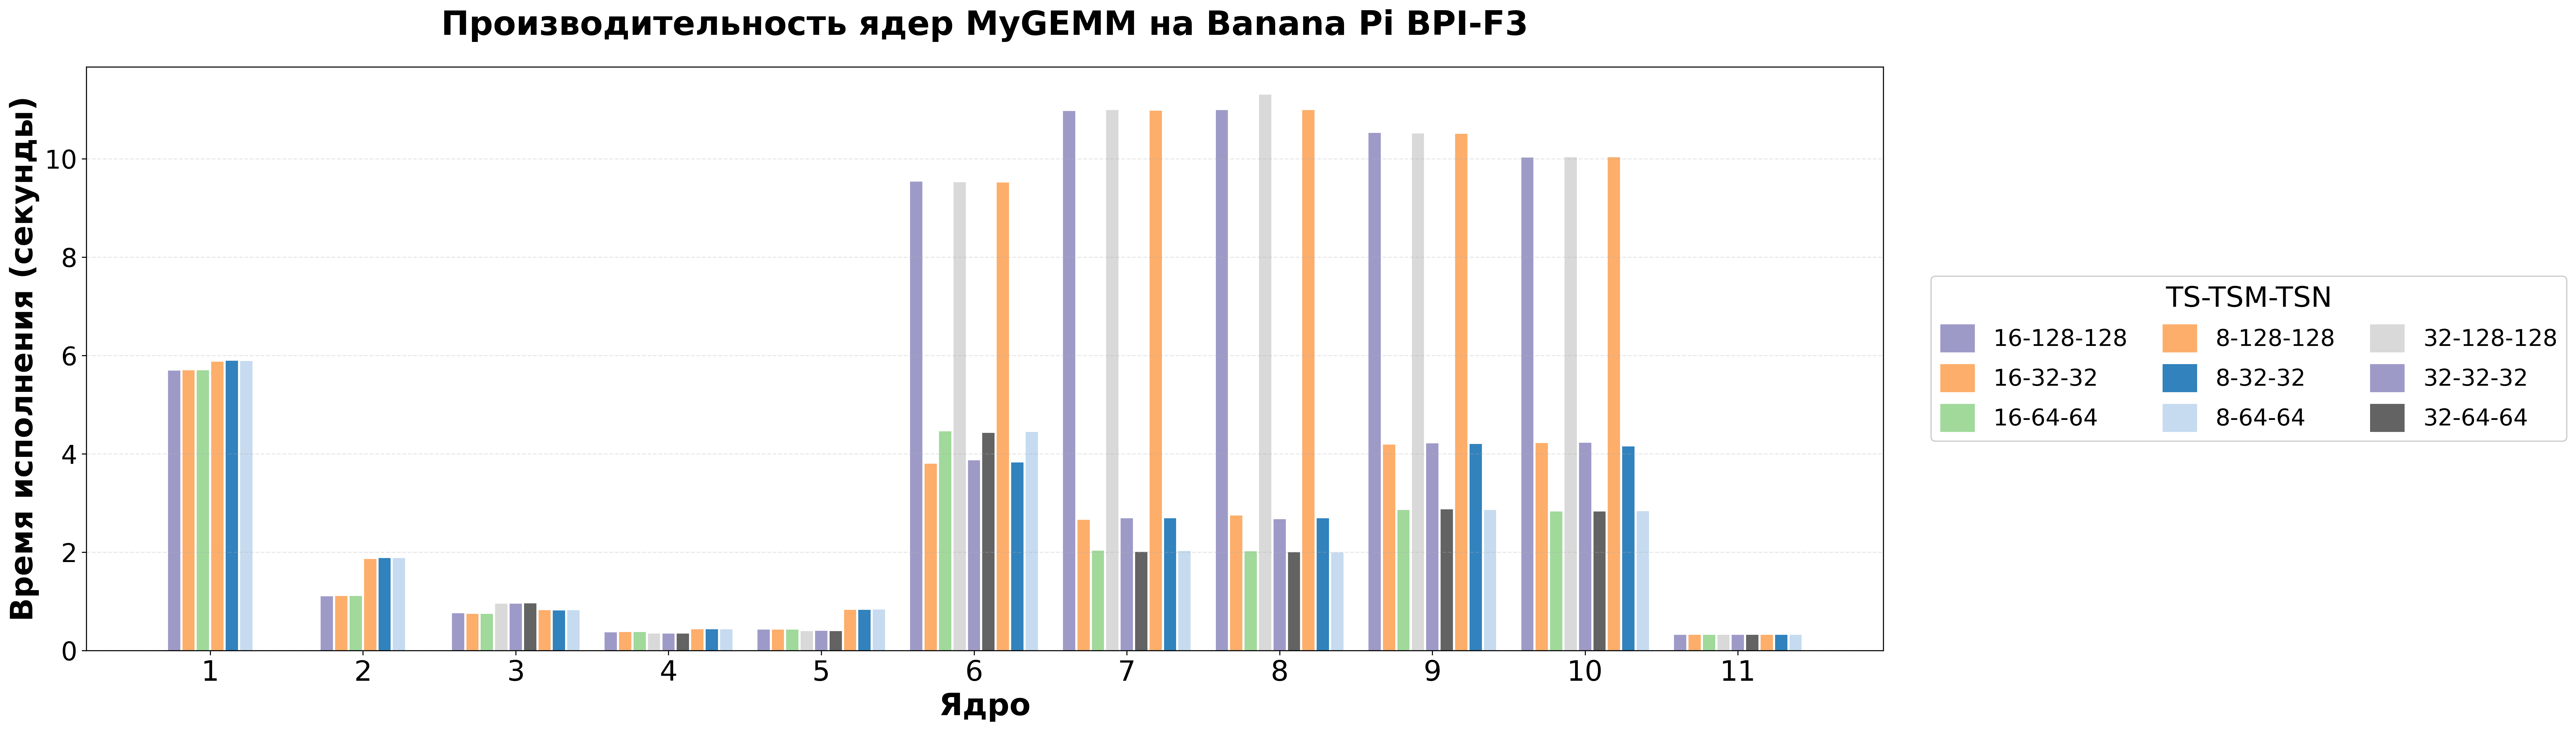
\includegraphics[width=1\textwidth]{figures/banana_pi.png}
\caption{Производительность ядер MyGEMM на платформе Banana Pi BPI-F3}
\label{fig:perf_bananapi}
\end{figure}

\begin{figure}[H]
\centering
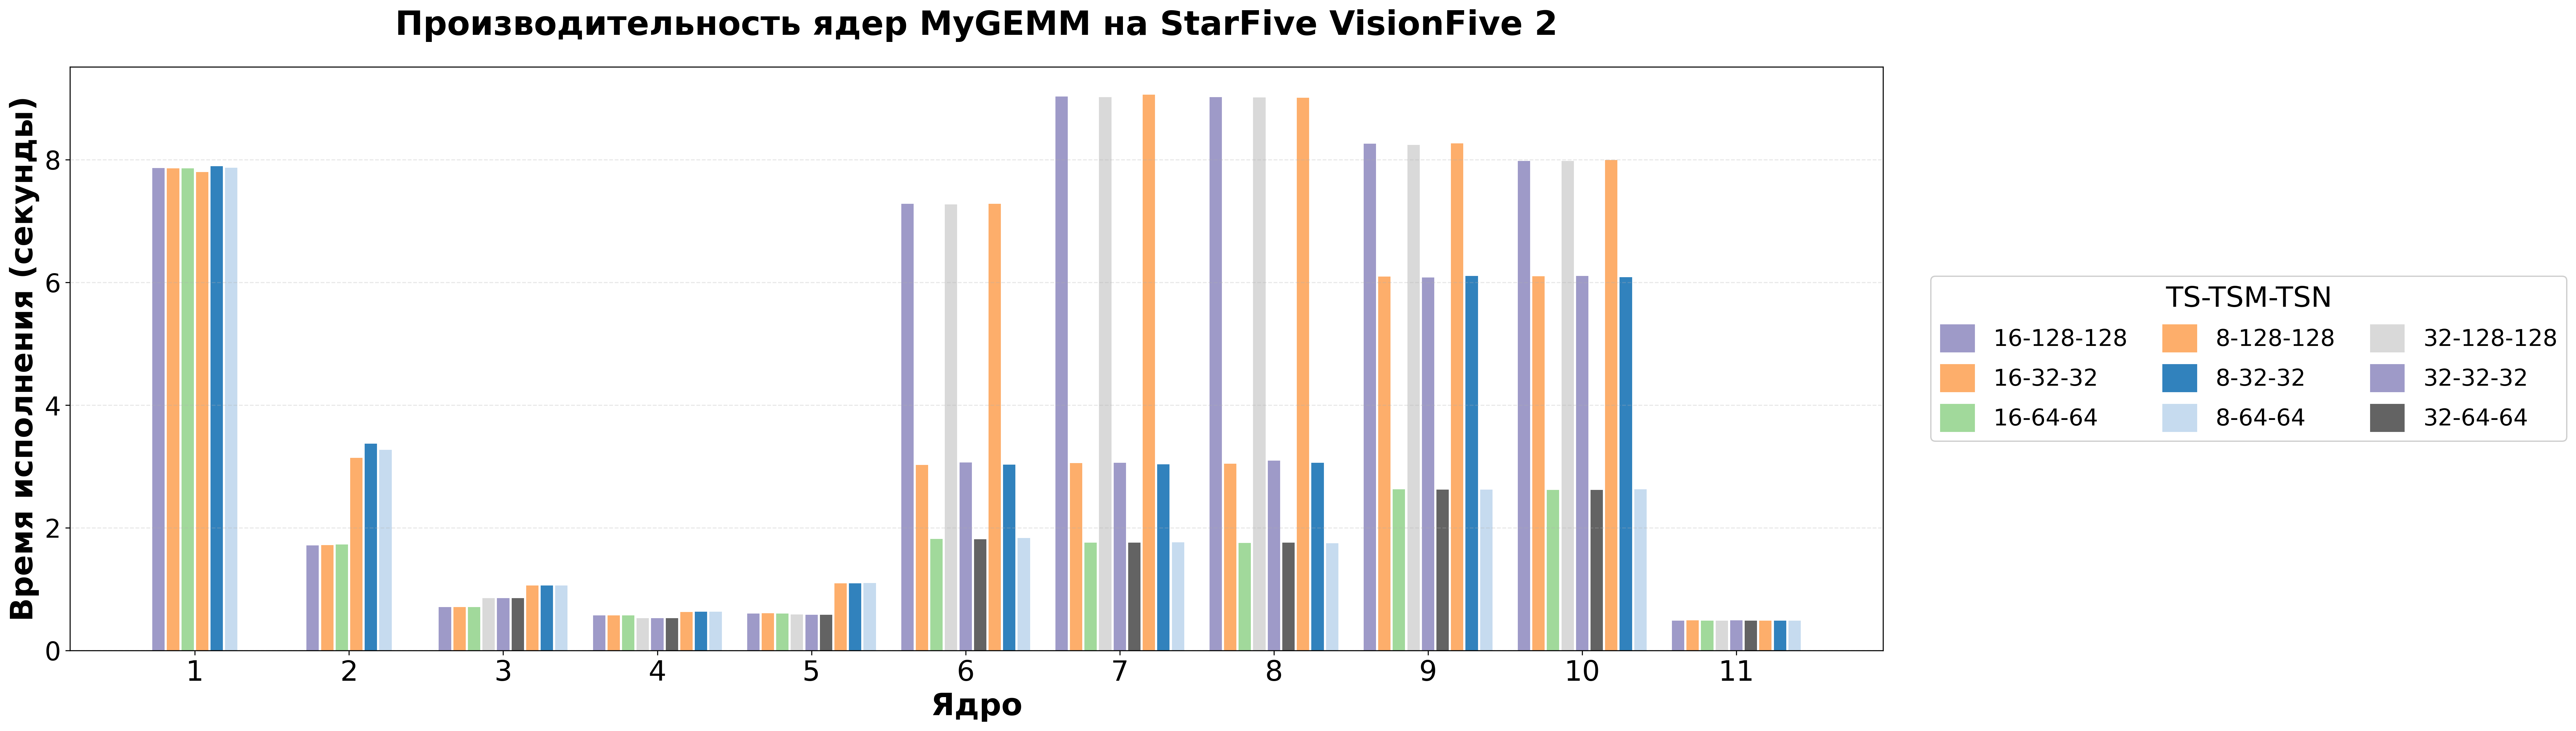
\includegraphics[width=1\textwidth]{figures/starfive.png}
\caption{Производительность ядер MyGEMM на платформе StarFive VisionFive 2}
\label{fig:perf_starfive}
\end{figure}

\begin{figure}[H]
\centering
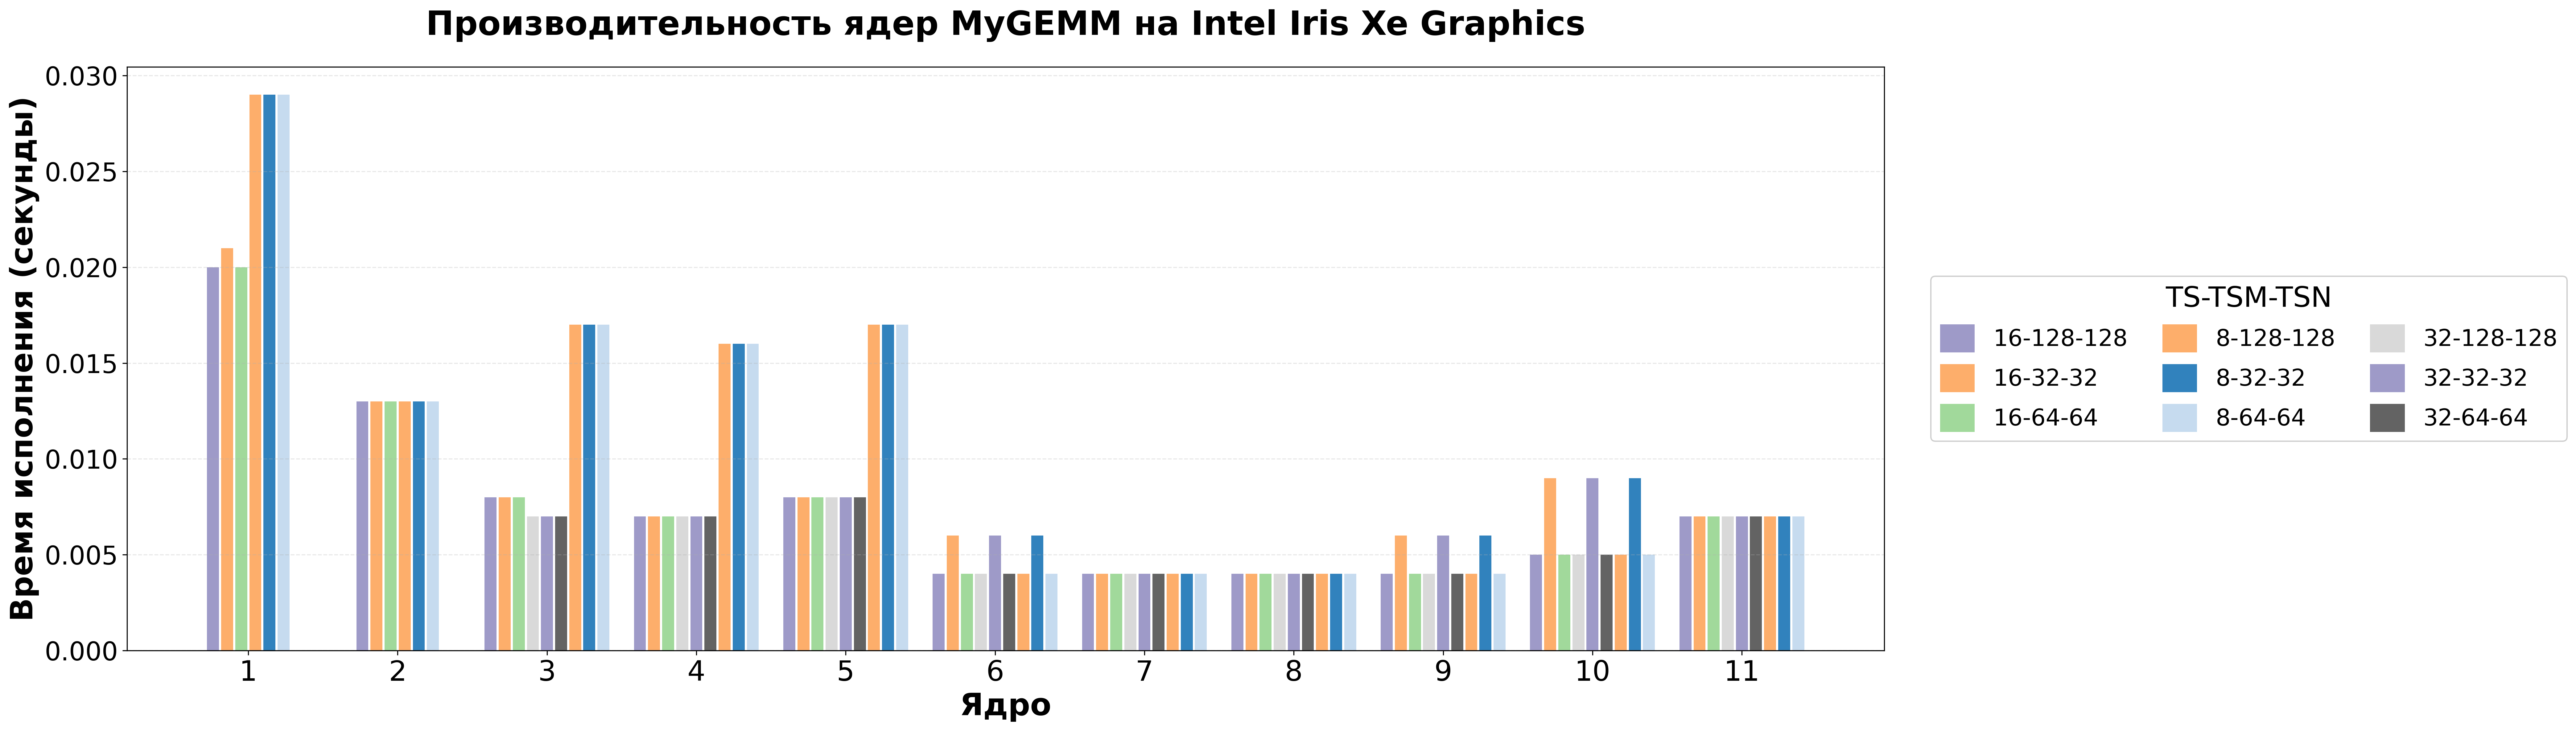
\includegraphics[width=1\textwidth]{figures/intel_xe.png}
\caption{Производительность ядер MyGEMM на референсной платформе Intel Iris Xe}
\label{fig:perf_intelxe}
\end{figure}

\subsubsection{Анализ результатов MyGEMM}

Экспериментальные данные демонстрируют значительные различия в производительности между RISC-V платформами и референсной системой Intel Iris Xe. Референсная платформа показывает время выполнения в диапазоне 0.004--0.029 секунд для различных ядер, что в среднем в 200--400 раз быстрее, чем RISC-V платформы.

Среди RISC-V платформ Banana Pi BPI-F3 демонстрирует лучшую производительность по сравнению со StarFive VisionFive 2, что объясняется более высокой тактовой частотой (2.0 ГГц против 1.5 ГГц) и большим количеством вычислительных ядер (8 против 4). Среднее время выполнения на Banana Pi составляет 0.3--11 секунд, на StarFive -- 0.5--9 секунд.

Ключевые наблюдения:

\textbf{Наилучший результат}. Ядро 11 (clBLAS-подход) демонстрирует наилучшую производительность на всех трёх платформах. На Banana Pi время выполнения составляет 0.32 сек (ускорение в 18.4 раза относительно наивной реализации), на StarFive -- 0.49 сек (ускорение в 16.1 раз), на Intel Iris Xe -- 0.007 сек.

\textbf{Проблемы векторизации}. Ядра 6--10, активно использующие векторизацию загрузки и записи данных, показывают неожиданно низкую производительность на RISC-V платформах. Время выполнения достигает 9--11 секунд, что в 10--30 раз медленнее более простых ядер 3--5. Разница в производительности между RISC-V и Intel для векторизованных ядер составляет 600--1000 раз, что указывает на серьёзные проблемы с реализацией векторных операций в драйверах OpenCL.

\textbf{Эффективность базовых оптимизаций}. Ядра 2--5 показывают хороший результат, достигая времени 0.3--0.6 секунд на RISC-V платформах, что в 10--25 раз быстрее наивной реализации.

\subsection{Результаты тестирования CLBlast}

После завершения процедуры тюнинга библиотеки CLBlast для обеих RISC-V платформ были проведены измерения производительности операции SGEMM. Для сравнения также были выполнены тесты на референсной платформе Intel Iris Xe с использованием предварительно натюненных параметров из базы данных CLBlast.

\subsubsection{Методология тестирования CLBlast}

Тестирование производительности CLBlast проводилось с использованием инфраструктуры matrix-benchmark, которая обеспечивает:

\begin{itemize}
    \item Автоматизированный запуск тестов для различных размеров матриц
    \item Сбор детальной статистики времени выполнения
    \item Вычисление производительности в GFLOPS
    \item Сравнение с другими библиотеками BLAS
\end{itemize}

Для каждого размера матрицы выполнялось 100 итераций операции умножения с последующим усреднением результатов. Тестировались квадратные матрицы размерами от $256 \times 256$ до $2048 \times 2048$ элементов с шагом 256.

\subsubsection{Результаты измерений CLBlast}

\textbf{[ЗДЕСЬ БУДУТ РАЗМЕЩЕНЫ ГРАФИКИ ПРОИЗВОДИТЕЛЬНОСТИ CLBLAST ПОСЛЕ ЗАВЕРШЕНИЯ ТЕСТИРОВАНИЯ]}

\begin{figure}[H]
\centering
% \includegraphics[width=1\textwidth]{figures/clblast_bananapi.png}
\caption{Производительность CLBlast на платформе Banana Pi BPI-F3 [График будет добавлен]}
\label{fig:clblast_bananapi}
\end{figure}

\begin{figure}[H]
\centering
% \includegraphics[width=1\textwidth]{figures/clblast_starfive.png}
\caption{Производительность CLBlast на платформе StarFive VisionFive 2 [График будет добавлен]}
\label{fig:clblast_starfive}
\end{figure}

\begin{figure}[H]
\centering
% \includegraphics[width=1\textwidth]{figures/clblast_intelxe.png}
\caption{Производительность CLBlast на референсной платформе Intel Iris Xe [График будет добавлен]}
\label{fig:clblast_intelxe}
\end{figure}

\subsubsection{Анализ результатов CLBlast}

\textbf{[РАЗДЕЛ БУДЕТ ДОПОЛНЕН ПОСЛЕ ЗАВЕРШЕНИЯ ТЕСТИРОВАНИЯ]}

Предварительные наблюдения:

\begin{itemize}
    \item Производительность CLBlast на RISC-V платформах после тюнинга
    \item Сравнение с лучшими ядрами MyGEMM (особенно ядро 11)
    \item Влияние автоматического тюнинга на производительность
    \item Масштабируемость на различных размерах матриц
\end{itemize}

\subsection{Сравнительный анализ MyGEMM и CLBlast}

\textbf{[РАЗДЕЛ БУДЕТ ДОПОЛНЕН ПОСЛЕ ЗАВЕРШЕНИЯ ТЕСТИРОВАНИЯ]}

\begin{table}[H]
\centering
\caption{Сравнение производительности лучших конфигураций MyGEMM и CLBlast [Данные будут добавлены]}
\label{tab:performance_comparison}
\begin{tabular}{lcccc}
\hline
\textbf{Платформа} & \textbf{MyGEMM (лучшее)} & \textbf{CLBlast} & \textbf{Разница} & \textbf{GFLOPS} \\
\hline
Banana Pi BPI-F3 & [TBD] с & [TBD] с & [TBD]\% & [TBD] \\
StarFive VisionFive 2 & [TBD] с & [TBD] с & [TBD]\% & [TBD] \\
Intel Iris Xe & [TBD] с & [TBD] с & [TBD]\% & [TBD] \\
\hline
\end{tabular}
\end{table}

Основные выводы из сравнительного анализа:

\begin{enumerate}
    \item Влияние автоматического тюнинга CLBlast на производительность RISC-V платформ
    \item Преимущества и недостатки каждого подхода
    \item Рекомендации по выбору библиотеки для различных сценариев использования
\end{enumerate}